\chapter{Adaptive Feature Specific Spectral Imaging-Classifier}\label{chap:Afssic}


\section{Motivation}

As I discussed in \Cref{chap:Introduction}, the spectrometer is one most of the widely used sensors in the history of mankind. This is because materials have unique spectra, by measuring the spectrum of a material and then comparing it to a database of known spectra one can quickly identify the test material. Spectrometers have become the main tool used for identifying materials for defense \cite{sun2004detection, pearman2006classification}, security \cite{liu2006detection, liu2007terahertz}, and medicine \cite{maquelin2000raman, maquelin2002identification}. 

By combining the spectrometer with the camera, the spectral imager produces a spectral datacube, a three dimensional representation of the scene consisting of two spatial dimensions and a spectral dimension ~\cite{garini2006spectral,eismann2012hyperspectral}.  By measuring both spatial and spectral information from an object scene, spectral imaging allows for improved discrimination of objects in a scene ~\cite{chang2003hyperspectral, ibrahim2010spectral, shaw2003spectral}. In this chapter, I will introduce the \acrfull{afssi-c}, a computational imaging system which directly computes the spectral classification at each spatial location in a scene.

One of the major design trade-offs of an \gls{isomorphic} spectral imaging sensor is that one must acquire a three-dimensional spectral datacube using a two-dimensional \gls{fpa} \cite{garini2006spectral}. Traditional isomorphic systems rely on a point-by-point acquisition technique to acquire the entire spectral datacube. A spotlight or whiskbroom technique simultaneously measures the entire spectrum from a single spatial location. This is repeated for each location until the spectral datacube is completely acquired \cite{wolfe1997introduction}. A pushbroom technique uses measures the spectrum of a spatial row (or column) in a two dimensional object scene at a time. This is repeated until all the rows (or columns) in the spectral datacube is acquired ~\cite{yang2003ccd, wolfe1997introduction}. A tunable filter technique, such as the Fabry-Perot interferometric filter \cite{fabry1897franges, perot1899application, fabry1901new}, simultaneously measures a single spectral channel but over the entire field-of-view, scanning through the spectral dimension~\cite{gat2000imaging} . 

A typical spectral datacube has a significant amount of measurement samples, for example, an airborne spectral imaging instrument called the  \gls{aviris} system, acquires $R_x \times R_y = 677$ spatial locations and $N_{\lambda} = 224$ spectral channels ~\cite{green1998imaging}, producing a spectral datacube with $N \approx 10^9$ measurement samples in $10$ minutes. 

Just like with the traditional spectrometer and camera, researchers have turned \gls{computational sensing} for spectral imaging. These architectures use the \gls{Fellgett advantage} (multiplexing) and \gls{Jacquinot advantage} (open aperture) to improve the \gls{snr} and use a computational step to reconstruct the spectral datacube \gls{spectralDataCube} from non-isomorphic measurements. Some spectral imaging architectures also leverage \gls{compressive sensing}. 

One of the early examples of computational sensing in spectral imaging is the \gls{ctis} \cite{descour1995computed}. The \gls{ctis} can reconstruct the spectral datacube \gls{spectralDataCube} from a single \gls{fpa} exposure by take multiple measurements of the spectral datacube simultaneously. The \gls{ctis} uses several gratings to create two-dimensional projections of the three-dimensional hyperspectral datacube. According to the central slice theorem, the two-dimensional Fourier Transform of each projection is a plane through the three-dimensional frequency space representing the spectral datacube. Ideally, one must collect enough projections to fully reconstruct the three dimensional frequency representation of the spectral datacube. The three-dimensional real-space distribution of the spectral datacube is thern recovered through an inverse 3D Fourier transform. However, in practice only a finite subset of projections are recorded and missing information is must be inferred. In the \gls{ctis}, the missing information is recovered by maximizing the likelihood of the measurement data using the expectation-maximization algorithm \cite{steven1993fundamentals, moon1996expectation}. The \gls{ctis} maybe considered compressive in that the number of measurement samples is less than the object dimensionality of the spectral datacube according to the practical definition of compressive sensing. However, it does not make any assumptions of sparsity or incoherence.

In another example of a computational sensing spectral imaging is the \acrfull{cassi} sensor. In the \gls{cassi}, a coded aperture and spatially codes the spectral datacube \gls{spectralDataCube}. The dispersive element then creates a projection of the spectral datacube that maps three-dimensional information into a two-dimensional image at the \gls{fpa}. Unlike the \gls{ctis}, only one two-dimensional projection is recorded per \gls{fpa} readout which allows for higher spatial resolution for the same detector array. Using calibration data and prior knowledge of sparsity, the post-processing step solves the \gls{lasso} problem to reconstruct the spectral datacube \cite{wagadarikar2008single, arce2014compressive}. Often a total-variation regularization is also invoked to improve reconstruction of the spatially varying image \cite{wagadarikar2008spectral, bioucas2007new}.

The task for most spectral imaging is material classification \cite{chang2003hyperspectral, dupont2011spatial, liu2014discriminative}. However the \gls{ctis}, the \gls{cassi}, and all other computational spectral imaging architectures use the post-processing step to reconstruct the spectral datacube \cite{hagen2013review}. Just like the traditional spectral imaging architectures, they produce a significant amount of data. Once the spectral datacube is reconstructed, the spectrum at each spatial location is compared to known spectra to make a classification. 

The \acrfull{afss} was the earliest known spectrometers to use the techniques of computational sensing for direct spectral classification \cite{dinakarababu2011adaptive}.

By utilizing adaptive spectral features and a sequential Bayesian update for hypothesis testing, the \gls{afss} significantly improves spectroscopic classification accuracy over traditional slit spectrometers without reconstructing the spectrum. 

The \gls{afssi-c} extends this concept first demonstrated by the \gls{afss} to spectral imaging. The \gls{afssi-c} directly classifies the spectrum at each spatial location with the reconstruction of the spectral datacube. By adopting a task-specific sensing approach, the \gls{afssi-c} greatly improves classification accuracy and simultaneous reducing transmission and storage requirements. Further more, the architecture of the \gls{afssi-c} leverages both the Fellgett and Jacquinot advantage like many other computational spectral imaging architectures utilizing significantly more light than the traditional systems mentioned above.



\section{Architecture}

Before discussing the architecture of the \gls{afssi-c} I want to quickly review the architecture of the \gls{afss}, is shown in \Cref{fig:afssArch}. Unlike the traditional slit spectrometer, the \gls{afss} images the dispersed slit onto a \gls{dmd}. The mirrors of the \gls{dmd} can then be adjusted to selectively reflect certain wavelengths towards the condensor lens, which then focuses light onto a single detector element \cite{dinakarababu2011adaptive}.

\begin{figure}
	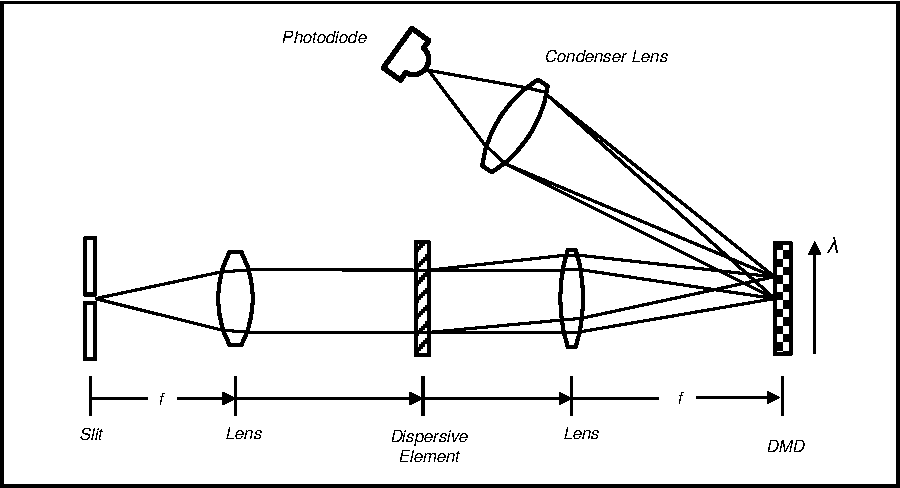
\includegraphics[scale=1.0]{afssArch}
	\captionof{figure}[The architecture of the Adaptive Feature Specific Spectrometer. ]{Blah blah blah.}
	\label{fig:afssArch}
\end{figure}

In order to create an imaging version of the \gls{afss}, one may attempt to extend the \gls{afss} architecture by simply forming an parallel array of \gls{afss} sensors to achieve classification across a spatial scene. However, like the proposed parallel single-pixel camera design in \Cref{chap:Scout}, this approach would significantly increases the \gls{swap-c} of the design. The \gls{afssi-c} provides a similar feature-based measurement approach and Bayesian framework but with a more compact architecture.

Rather than a fully parallel version of the \gls{afss}, the optical design of the \gls{afssi-c} uses a single \gls{dmd} and a single set of lenses and dispersive elements. Not only does this approach share resources across multiple spatial locations, it avoids the expense of pixel-specific components.


\begin{figure}
	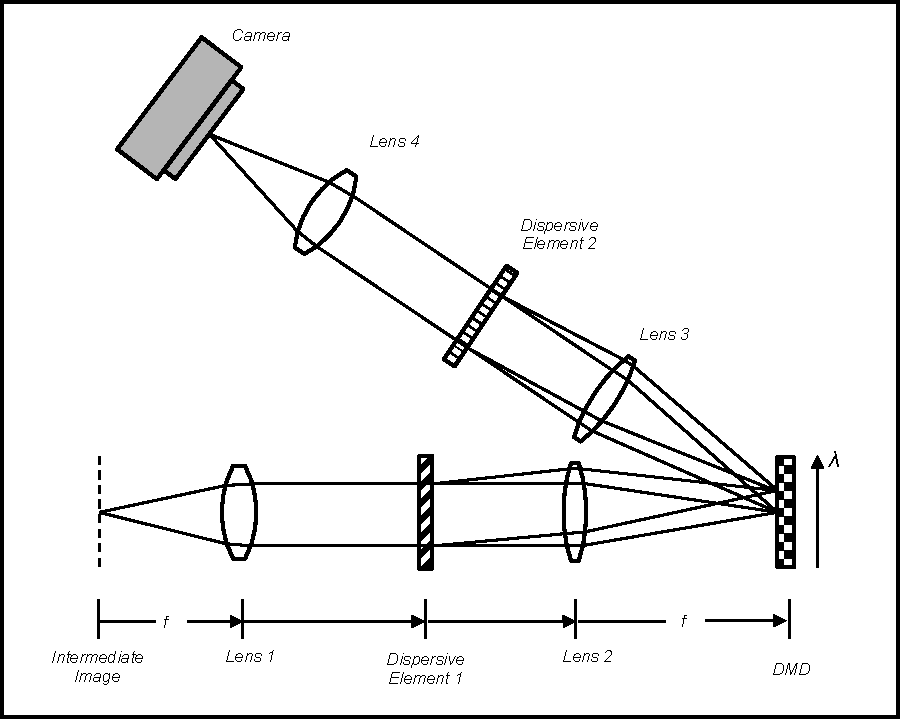
\includegraphics[scale=1.0]{afssicArch}
	\captionof{figure}[The architecture of the Adaptive Feature Specific Spectral Imaging-Classifier]{An objective lens forms the intermediate image of the object scene at the input plane of the instrument. The first lens collimates the light and a diffraction grating disperses the light. A second lens images spectrally dispersed versions of the image of the object scene onto the \gls{dmd}. The \gls{dmd} directs light to a beam dump or reflects the light towards the third lens on a mirror-by-mirror basis. Collimated light from third lens
is sent through a second grating, and finally imaged onto the detector by the fourth lens.}
	\label{fig:afssicArch}
\end{figure}


The design of the \gls{afssi-c} is essentially two 4\textit{f} open-aperture monochromators back-to-back, shown in Fig.~\ref{fig:afssicArch}. A \gls{dmd} divides the two halves. An objective lens (not shown) creates an intermediate image at the input plane of the instrument. At this point in the system one can imagine the source spectral datacube as depicted in \Cref{fig:sysCubes}(a), where $x$ and $y$ are the spatial axes, and $\lambda$ the spectral axis. The first lens of the system collimates the light. The first grating disperses the light. The second lens then images spectrally dispersed copies of the intermediate image at the \gls{dmd}. Just prior to being reflected from the \gls{dmd}, one can imagine the spectral datacube as being sheared at an angle in the direction of the dispersion, see \Cref{fig:sysCubes}(b). 
%
%
\begin{figure}
	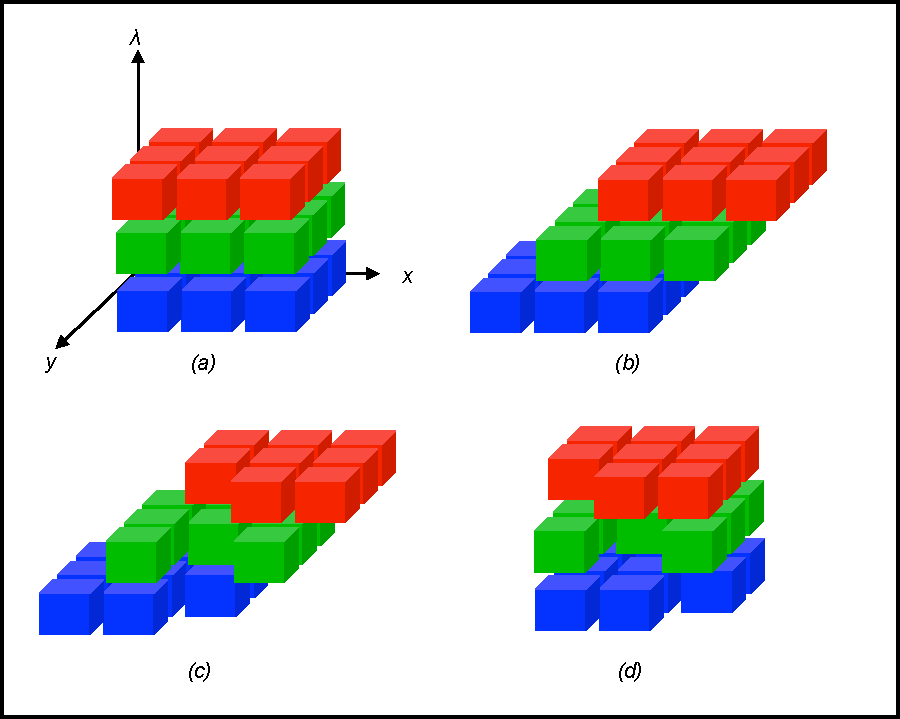
\includegraphics[scale=1.0]{justCubes}
	\captionof{figure}[Visualization of datacube progression through the \gls{afssi-c} system.]{(a) The input cube is (b) sheared by the first grating, (c) encoded at the \gls{dmd}, and finally (d) spatially re-registered by the second grating.}
	\label{fig:sysCubes}
\end{figure}
%
%
We implement mirror patterns on the dense array of micromirrors at the \gls{dmd} which either allow the light to continue to the rest of the system, or block it by sending it to a beam dump, on a mirror-by-mirror basis. This pattern encodes the datacube, portrayed in \Cref{fig:sysCubes}(c) as holes punched through the sheared cube.

The now-encoded signal is once again collimated before hitting the second grating, which is identical to the first, but with the dispersion direction flipped so as to undo the applied dispersion. This removes the shear in the encoded spectral datacube, as depicted in \Cref{fig:sysCubes}(d). The final lens in the system focuses that result onto the detector array, which integrates the cube through the spectral dimension. The result at each pixel is the inner product of the source spectrum at that location in the scene with a spectral filter---the implemented feature vector---imposed on that location by the mirror pattern on the \gls{dmd}.

We chose to use a dual-disperser (DD) architecture rather than the single-disperser architecture such as the one in the \gls{cassi} since the mirror patterns on the \gls{dmd} acts as spectral filters for each spatial location. In the single-disperser design the spatially-varying spectral encoding is more appropriate for parallel direct classification, as the measurements can be mapped one-to-one with the spatial locations in the scene, allowing for parallel operation of the Bayesian inference approach, rather than having to solve a single larger joint inference problem.

The mirror pattern at the \gls{dmd} gives rise to the spectral filters that act at each spatial location in the scene. We turn to a system model to understand this relationship.
The system model, and the relationship between the pixelation of the detector and the pixel size at the \gls{dmd}. We start with this model, and extend it to provide the restriction imposed on the feature design.

\subsection{Forward Model}

If we consider a source spectral density of $S_0 \left(x, y;\lambda \right)$ at the input aperture and assume unit magnification throughout the optical system, we can write the measurements at location $(n,l)$ on the detector array as
%
\begin{align} \label{eq:PixelizedDetectIntensity}
	\Gamma_{nl} &= \sum_{n^\prime l^\prime} \iiint \mbox{rect} \left( \frac{x}{\Delta} - l, \frac{y}{\Delta} - n \right) \mbox{rect} \left( \frac{x-\alpha \left(\lambda - \lambda_c\right)}{\Delta} - l^\prime , \frac{y}{\Delta} - n^\prime \right) \notag \\
 	&\qquad \times T_{n^\prime l^\prime} S_0 \left( x, y; \lambda \right) dx \, dy \, d\lambda.
\end{align}
%
where $\Delta$ is the pixel (mirror) size on the \gls{dmd} and the \gls{fpa}, $T$ is an array that describes the pixelated  mirror pattern on the \gls{dmd},  $\alpha$ is the linear dispersion of the gratings, and $\lambda_c$ is the center wavelength of the system. The first rectangular function represents the finite pixel size of the \gls{fpa} at pixel coordinates $(n,l)$. The second rectangular function represents how the spectral density is sheared: each  value of $x$ is shifted the amount corresponding the distance $\alpha \ap{\lambda - \lambda_c}$. 



As will be shown later, the system relies on calibration which accommodates deviations from these assumptions.

If we analyze two constrained cases, we can gain an understanding of how the spectral filter influences the measured intensity.
We first consider a monochromatic source $S_0 \left(x, y, \lambda\right) = I_0 \left(x, y \right) \delta \left( \lambda - \lambda_c \right)$, where $I_0$ is the intensity distribution of the monochromatic scene. In this case, Eq.(\ref{eq:PixelizedDetectIntensity}) simplifies to
%
%
\begin{align} \label{eq:MonoChrome}
\Gamma_{nl} \left(\lambda = \lambda_c \right) &= \sum_{ n^\prime l^\prime} \iiint \mbox{rect} \left( \frac{x}{\Delta} -  l, \frac{y}{\Delta} - n \right)  \mbox{rect} \left( \frac{x}{\Delta} - l^\prime, \frac{y}{\Delta} - n^\prime \right) \notag \\
 &\qquad \times T_{n^\prime l^\prime} I_0 \left( x, y \right) \delta \left( \lambda - \lambda_c \right) dx \, dy \, d\lambda  \notag \\
 &= \sum_{n^\prime l^\prime} \delta_{ll^\prime} \delta_{nn^\prime} T_{n^\prime l^\prime} I_{nl} \notag \\
 &= T_{nl} I_{nl},
\end{align}
%
%
where $I_{nl}$ is a spatially pixelated version of the monochromatic source with intensity distribution $I_0 \left(x, y \right)$

Now we consider a case with the monochromatic source is shifted by a spectral channel $\Delta \lambda = \Delta / \alpha$. Then,
%
\begin{align} \label{eq:Mono2}
	\Gamma_{nl}\left(\lambda = \lambda_c + \Delta \lambda\right) &= \sum_{l'n'} \iiint \mbox{rect} \left( \frac{x}{\Delta} - l, \frac{y}{\Delta} - n \right)  \mbox{rect} \left( \frac{x}{\Delta} - \left(l' + 1 \right), \frac{y}{\Delta} - n' \right) \notag \\
 	&\qquad \times T_{n'l'} I_0 \left( x, y \right) \delta \left( \lambda - \left( \lambda_c + \Delta \lambda \right)\right) dx \, dy \, d\lambda  \notag \\
 	&= \sum_{n'l'} \delta_{ll'} \delta_{nn'} T_{n' \left( l' + 1 \right)} I_{nl} \notag \\
 	&= T_{n\left(l - 1 \right)} I_{nl}
 \end{align}
%
where we find that a shift by a spectral channel results in a shift in the mirror pattern.

For a natural scene with content spanning the spectral range, we can consider spectral channel index $\kappa$ out of $C$ total spectral channels.
We can also define a discretized source spectral datacube $S_{nl\kappa}$, and then the detector signal $\Gamma_{nl}$ as a result of mirror pattern $T$ acting on the pixelated source is
%
%
\begin{equation}
	\Gamma_{nl} = \sum^{C-1}_{\kappa = 0} T_{n \left( l + \kappa \right)} S_{nl\kappa},
\end{equation}
%
%
which shows the measurement at each pixel being the inner product of the source spectrum and the feature vector which results from the mirror pattern. If we look at an adjacent pixel on the detector, $\Gamma_{n \left(l +1 \right)}$ we find that
%
%
\begin{equation}
\Gamma_{n\left(l-1\right)} = \sum^{C-1}_{\kappa = 0} T_{n\left( l + 1 + \kappa \right)} S_{n\left(l+1\right)\kappa}.
\end{equation}
%
%
The spatial location $\left(n,l \right)$ sees the effect of the pattern in mirror locations $T_{nl}$ to $T_{n\left(l+C-1\right)}$, while the neighboring spatial location at $n, \left( l + 1\right)$ is encoded by the mirror pattern from $T_{n\left(l+1\right)}$ to $T_{n\left(l + C \right)}$. What we notice is that the mirror pattern for neighboring pixels overlap, and have the mirror pattern from $T_{n\left( l + 1 \right)}$ to $T_{n\left(l + C - 1 \right)}$ in common. Essentially what each source location sees is a spectral filter formed by a length $C$ segment of a mirror pattern which spans the entire row, with the neighboring location seeing a length $C$ segment of that underlying pattern offset by 1.

\subsubsection{Simple Example}

Imagine a spectral datacube with dimensions $R_x \times R_Y \times R_\lambda = 2 \times 2 \times 2$. Thus the spectral datacube has two discrete spatial locations in the $x$ and $y$ direction. Also imagine that the \gls{fpa} has a readout resolution of $r_x \times r_y = 2 \times 2$

The overlap of the spatial and spectral information at the \gls{dmd} disallows independent feature vectors for each spatial location. The spectral filters imposed by the \gls{dmd} pattern are unique for every spatial location, but \textit{cannot} be implemented independently, requiring the features to be designed \textit{jointly} for spatial locations along a row.



\section{Adaptive Classification Algorithm}


The \gls{afssi-c} uses adaptive features designed from information in previous measurements to make a classification decision from hypothesis spectra in a spectral library. This library is common to all spatial locations, and it is helpful to first look at the process of feature design and classification decision for a single spatial location. We can then expand the analysis to include the entire scene, building from the single-location tool set.

The measurement at each detector pixel is compared to the spectral library, subject to the spectral filter implemented at that spatial location. A probability is assigned to each hypothesis in the library using Bayes' theorem. The conditional probability of hypothesis $\textbf{h}_i$ given the measurement history up to the $k^{th}$ measurement $\{m\}_k$, can be written as:
%
\begin{equation}\label{eq:BayesThm}
\mbox{P} \left( \textbf{h}_i | \{ m \}_k \right) = \frac{\mbox{P} \left( \{m\}_k |\, \textbf{h}_i \right) \; \mbox{P} \left(\textbf{h}_i\right)}{\mbox{P} \left( \{m\}_k \right)}.
\end{equation}

The probabilities are assigned and updated using a Gaussian noise model and log-likelihood ratios, as implemented by the AFSS in \cite{AFSSbetter}. The probability assignment is on a per-pixel basis and is independent of the probability assignment of adjacent spatial locations in the \gls{afssi-c}.

Features are designed to yield measurements which discriminate between the hypotheses with the greatest probability. To this end we use a modification of principal component analysis (PCA) that employs the updated probability estimates of each hypothesis as a weighting factor. We consider this an intuitively reasonable approach, keeping in mind that the first principal component (PC) is an eigenvector of the scatter matrix, along the direction of greatest variance in the library spectra~\cite{PCAwiley}. By taking the inner product of the spectra at each location with this first eigenvector, we significantly separate the possible measurement outcomes, facilitating discrimination. Using standard PCA does not allow for informing subsequent measurements with previous results, so we modify PCA as follows.

At each individual pixel we create a scatter matrix with $R$ spectral hypotheses, with individual spectrum $\textbf{s}_r$, weighted in relation to the prior probability associated with each hypothesis given the measurement history. The individual scatter matrices $\textbf{{Q}}(k)$ at each spatial location with spectral library element hypothesis $\textbf{h}_r$ take the form
%
%
\begin{align}
\textbf{Q}(k) &= \sum^R_{r \;= \,1} \mbox{P} \left( \textbf{h}_r | \{m\}_k \right) \left(\textbf{s}_r - \bar{\textbf{s}} \right) \left(\textbf{s}_r - \bar{\textbf{s}} \right)^T \notag \\
&=\textbf{X}(k)\;\textbf{X}^T(k). \label{eq:preScatter}
\end{align}
%
%
Here $\textbf{X}(k)$ is the matrix of weighted spectral elements, where the row index $i$ is from 1 to the number of spectral channels $C$, with columns $j$ from 1 to $R$ as follows,
%
%
\begin{equation}
	\textbf{X}_{i j}(k) = \sqrt{\mbox{P} \left(\textbf{h}_j \vert \{m\}_k \right)} \left(\textbf{s}_{i j} - \bar{\textbf{s}}_i\right),
\end{equation}
%
%
and $\bar{\textbf{s}}$ is the probabilistically-weighted sum of the spectral library:
%
%
\begin{equation} \label{eq:Sbar}
\bar{\textbf{s}} = \sum^R_{r \;= \, 1} \mbox{P} \left( \textbf{h}_r | \{m\}_k \right) \textbf{s}_r.
\end{equation}


We can then compute the first eigenvector of $\textbf{Q}(k)$, analogous to PCA. We call this probabilistic-PCA or pPCA, and in the case of the AFSS this eigenvector becomes the feature for the next measurement. The scatter matrix $\textbf{Q}(k)$ is then updated with every measurement.


The effect this has on the first PC is illustrated in the two-dimensional (i.e. a spectral library with two spectral channels) example in Fig.~\ref{fig:pPCA}. In Fig.~\ref{fig:pPCA} (a) each hypothesis is equiprobable, whereas in Fig.~\ref{fig:pPCA}(b) the  hypotheses  are probabilistically-weighted after the first measurement, showing a new direction for the first PC vector. In the case of the AFSS~\cite{AFSSbetter}, the features derived from this PC vector allow the system to further discriminate between the most likely library spectra when making a classification decision.

% pPCA example figure - single pixel
%
%
\begin{figure}[htb]
  \centering
  % Requires \usepackage{graphicx}
  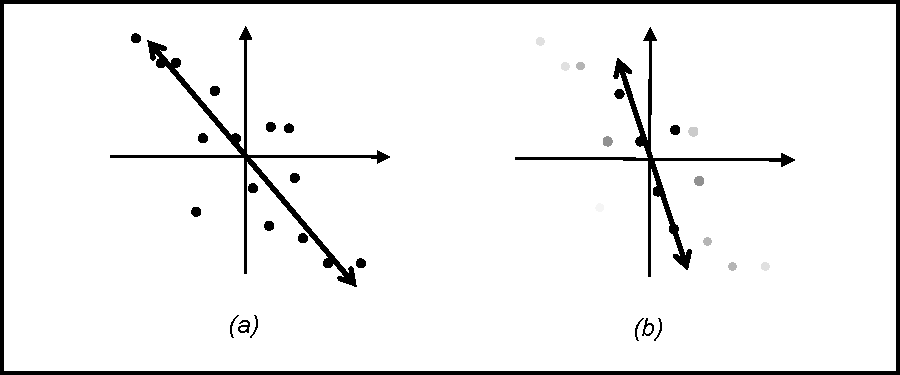
\includegraphics[scale=1.0]{pPCA}
  \caption{Depiction of the pPCA (simple 2D example). (a) First principal component before a measurement has been made. All of the hypotheses are equiprobable, depicted here as all points having the same grayscale value. (b) After a measurement has been made: the darker points are more probable hypotheses, with the less probable hypotheses taking on lighter shades of gray. The first principal component has now been shifted to the direction of greatest variation in the weighted data.}\label{fig:pPCA}
\end{figure}
%
%
%Before moving into joint feature design, we highlight the pertinent aspect of the single pixel feature design scheme upon which joint feature design is built.
%Figure \ref{jointpPCA} (a) is a cartoon of the steps involved to illustrate the generation of the matrix $\textbf{X}(k)$ from Equation (\ref{preScatter}). The source spectra $\textbf{s}_r$ (1) is centered around the mean %$\left(\textbf{s}_r - \bar{\textbf{s}}\right)$ (2), and finally multiplied by the probability of each hypothesis spectrum, illustrated by the variation in the thickness of the plot lines (3).

As discussed above, the \gls{afssi-c} system architecture mixes spatial and spectral information at the coding plane in a way that requires joint design of the mirror pattern on each row. Therefore, pPCA is further modified by instead using the matrix $\textbf{\~X}_{u v}(k)$, constructed from the single-location probabilistically weighted hypothesis matrices $\textbf{X}_{ij}(k)$ from each spatial location ($l^\prime$) in a row ($n^\prime$). The individual $\textbf{X}_{i j}(k)$ matrices become block elements in this much larger matrix, with each block offset in $v$ by the appropriate value of $l^\prime$. The $\textbf{X}_{ij}(k)$ matrices for neighboring spatial locations share $C-1$ columns in this larger matrix, which represents the overlap of spatial and spectral information at the \gls{dmd} as illustrated by the system model discussion. Figure \ref{fig:jointpPCA}(b) illustrates the stacking of the elements of the mean-centered, weighted library spectra from Fig. \ref{fig:jointpPCA}(a) into a larger array $\textbf{\~X}(k)$. We arrive at a joint scatter matrix similar in form to Equation (\ref{eq:preScatter}),
%
%
\begin{equation}
	\textbf{\~{Q}}(k) = \sum^{\tilde{R}}_{\tilde{r}=\,1} \left(\textbf{\~x}_{\tilde{r}}(k) - \bar{\textbf{\~x}}(k)\right) \left(\textbf{\~x}_{\tilde{r}}(k) - \bar{\textbf{\~x}}(k)\right)^T,
\end{equation}
%
%
where $\bar{\textbf{\~x}}$ is the mean of each column in $\textbf{\~X}$, and the sum is over the library elements $\tilde{r}$ from all of the row locations. The first PC of $\textbf{\~Q}(k)$ is a vector pointing in the direction of greatest variation in the probability-weighted data for the entire row. We repeat this process for all of the rows in the datacube to arrive at the features to be implemented for the subsequent measurement. We refer to this feature design method as joint-pPCA.

With the system able to take advantage of prior information to adapt features for the subsequent measurement, the \gls{afssi-c} is able to accurately and rapidly determine pixel-level classification. For this work, the classification decision after each measurement is given by the maximum a-posteriori probability (MAP) estimate (the mode of the probability mass function)\cite{poor2013introduction} of the hypothesis spectra at each location. We now look at the components and design of the experimental system. 


% joint-pPCA figure
\begin{figure}[htb]
	\centering
	\includegraphics[height=3in]{jointpPCA}\\
	\caption{Joint-pPCA schematic. (a) The pictorial illustration of the formation of $\textbf{X}(k)$ from Equation(\ref{eq:preScatter}). The hypothesis spectra (1) are centered around the mean (2), and given a weight based on their probabilities (3).  (b) The joint-pPCA calculation involves the stacking of the $1, \ldots, C-1$ elements of $\textbf{X}_{i, j}(k)$ for each location $\left( n^\prime,\;l^\prime \right)$ along a row into a larger matrix $\textbf{\~X}_{uv}(k)$. The final joint-pPCA scatter matrix is formed from $\textbf{\~X}(k)$ multiplied by its mean-centered transpose, to arrive at scatter matrix $\textbf{\~Q}(k)$. The first principal component of this much larger scatter matrix is then in the direction of greatest variation in the joint-position data.}\label{fig:jointpPCA}
\end{figure}



\section{Experiments}

The goal of the \gls{afssi-c} effort was to design and build a system that would yield direct classification and outperform traditional spectral imaging systems in classification accuracy. This comparison is to be performed via simulation, so we must validate our ability to simulate the real world performance of such a system. Thus, we first compare the experimental results of the \gls{afssi-c} system (Fig. 5) with simulation. This allows for confident comparison to the conventional approaches.

To be convinced in our experimental corroboration of the simulation results, we need to be able to claim agreement for different levels of classification difficulty. To this end, we corrupt the experimental measurements in software with white Gaussian noise, and hence we manipulate the difficulty of classification. As in [32], the experimental results reported here are for a 4-class problem, with an input spectral datacube of $64 \times 64$ spatial pixels and 38 spectral channels. Figure 6 is an illustration of the spectral source used, with the associated 4-class spectral library.

% joint-pPCA figure
\begin{figure}[htb]
	\centering
	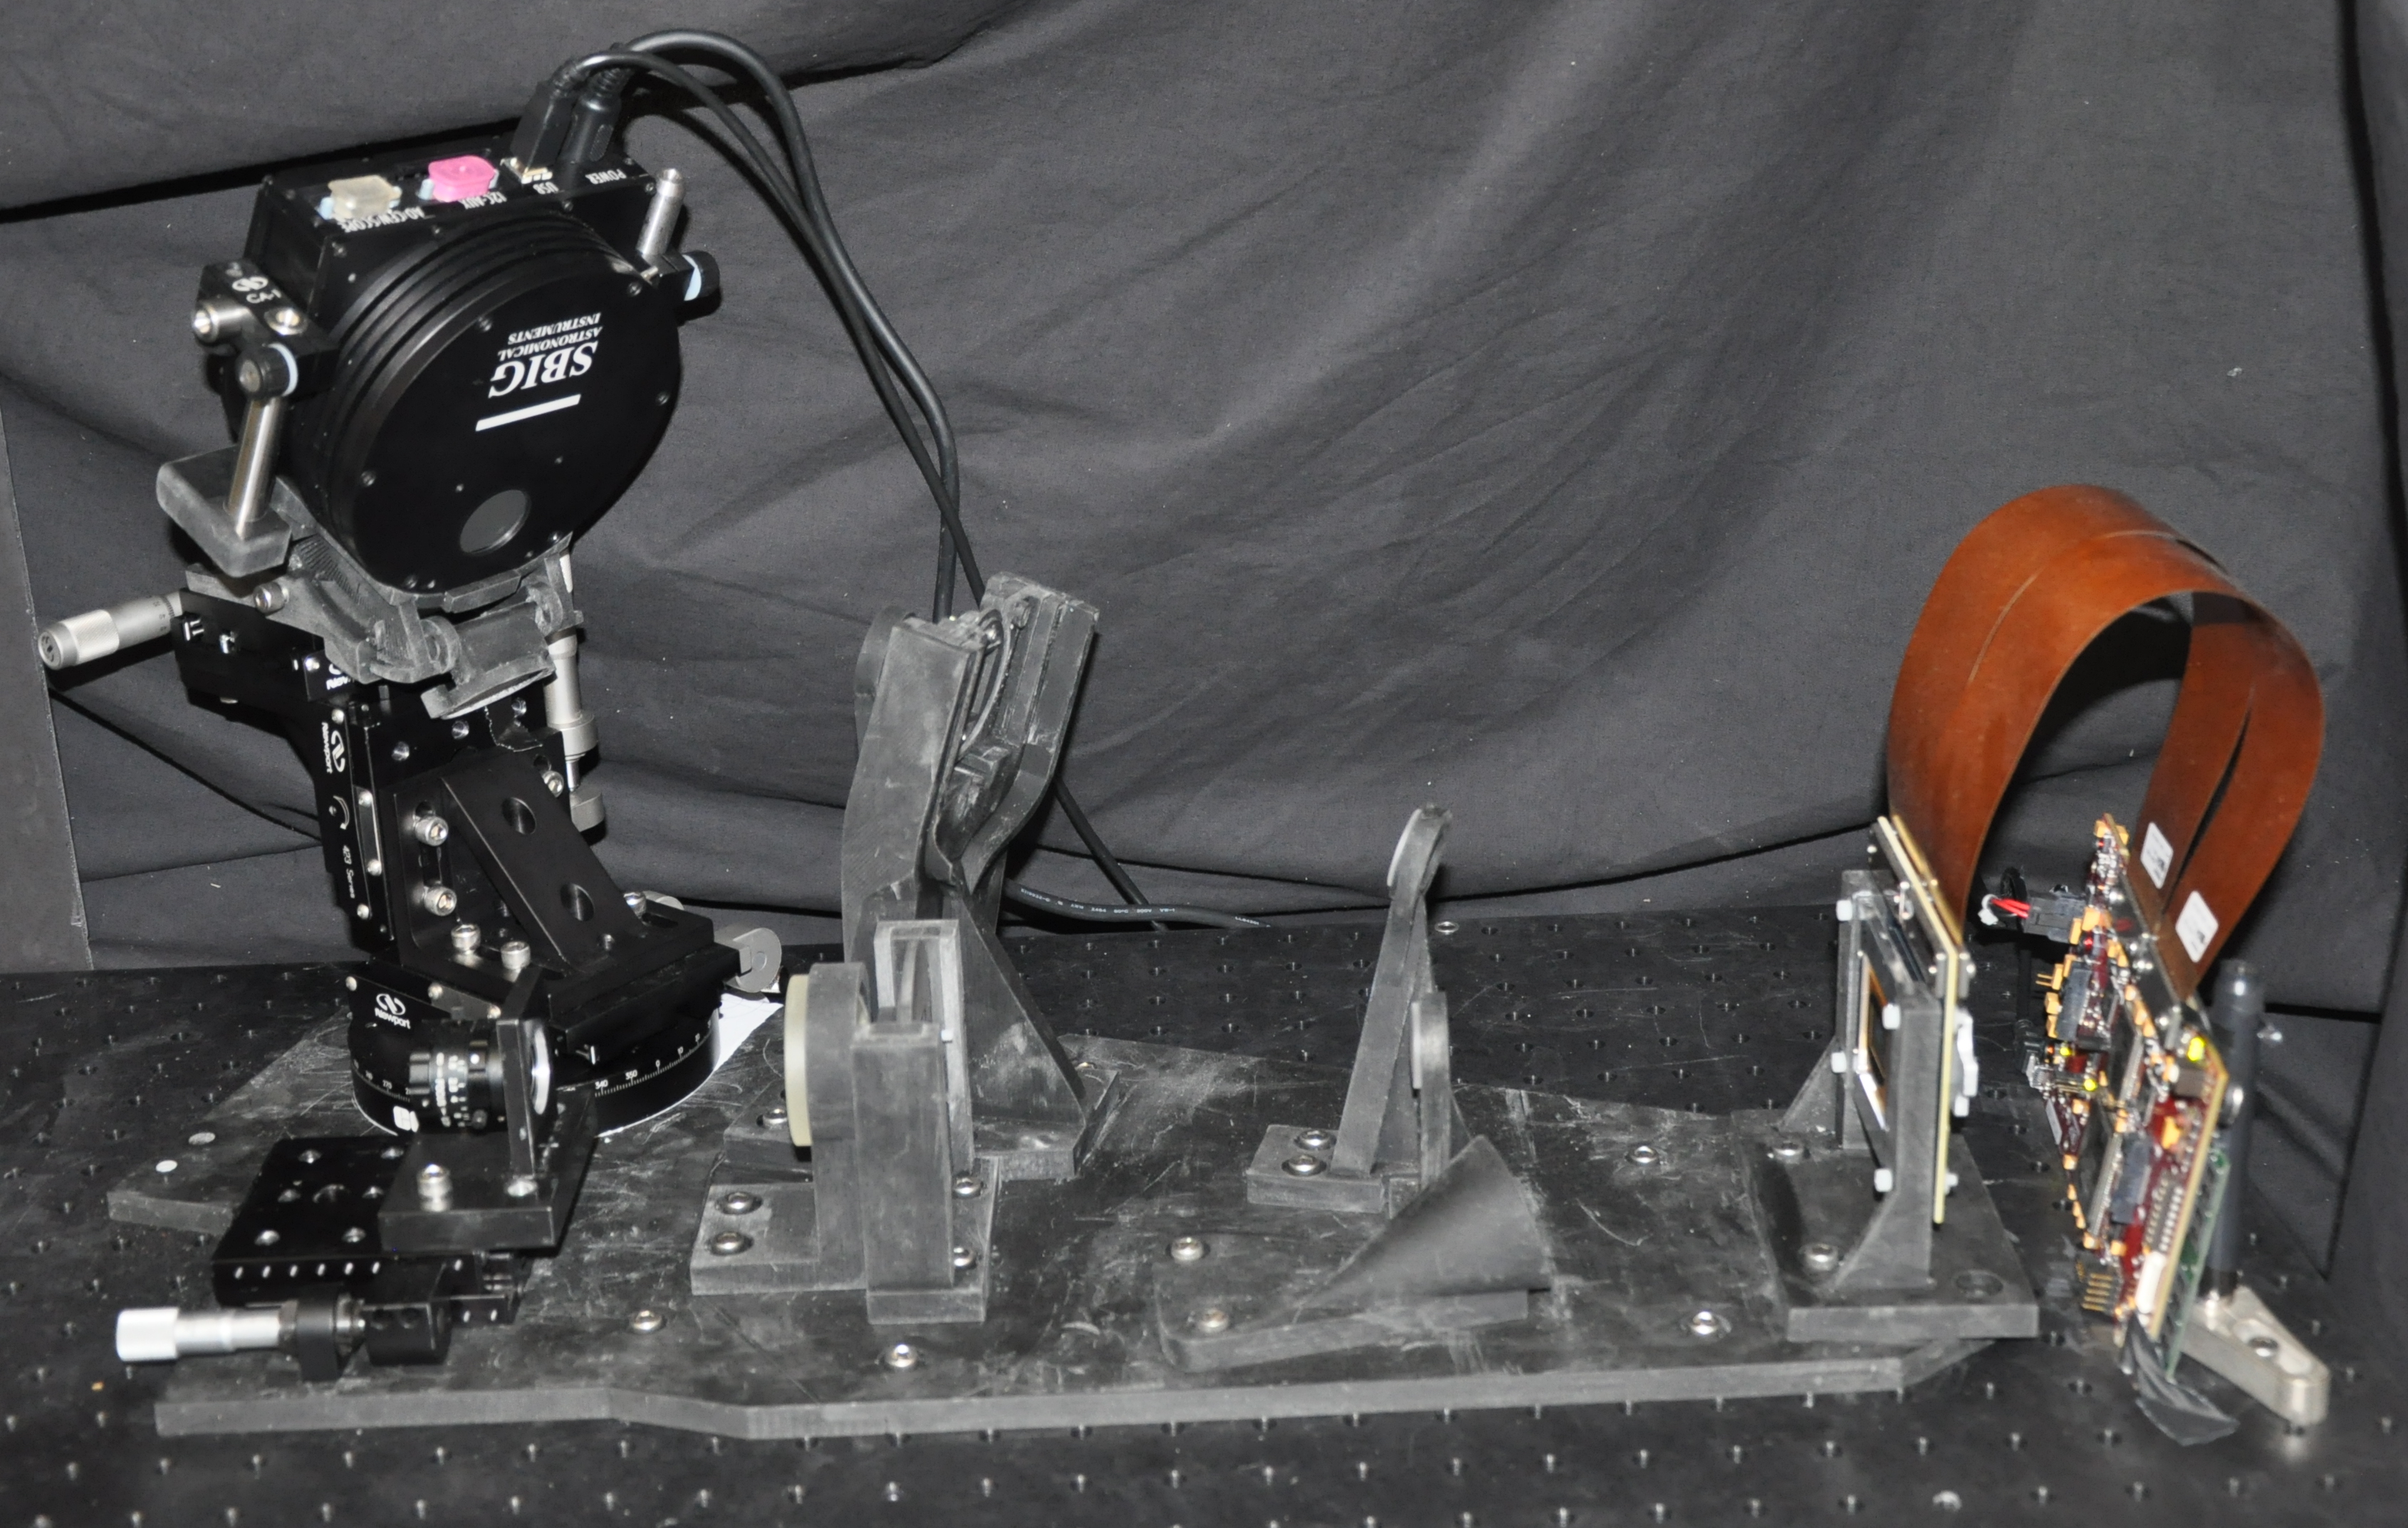
\includegraphics[height=3.7in]{afssicPhoto1.JPG}\\
	\captionof{figure}[Photograph of AFSSI-C.]{Photo of \gls{afssi-c}}
	\label{fig:afssicPhoto1}
\end{figure}


While this spectral datacube is small compared to those used in remote sensing, the implemented size was driven by practical considerations regarding the source, \gls{dmd} and detector on hand. The dual-disperser architecture, in general, places no significant limitation on possible datacube sizes. Similarly, the processing involved in the Bayesian inference and feature design are computationally lightweight and do not create a computational limit on datacube size.

% Plot of the \gls{afssi-c} 4 Class Spectral Library
\begin{figure}[htb]
	\centering
	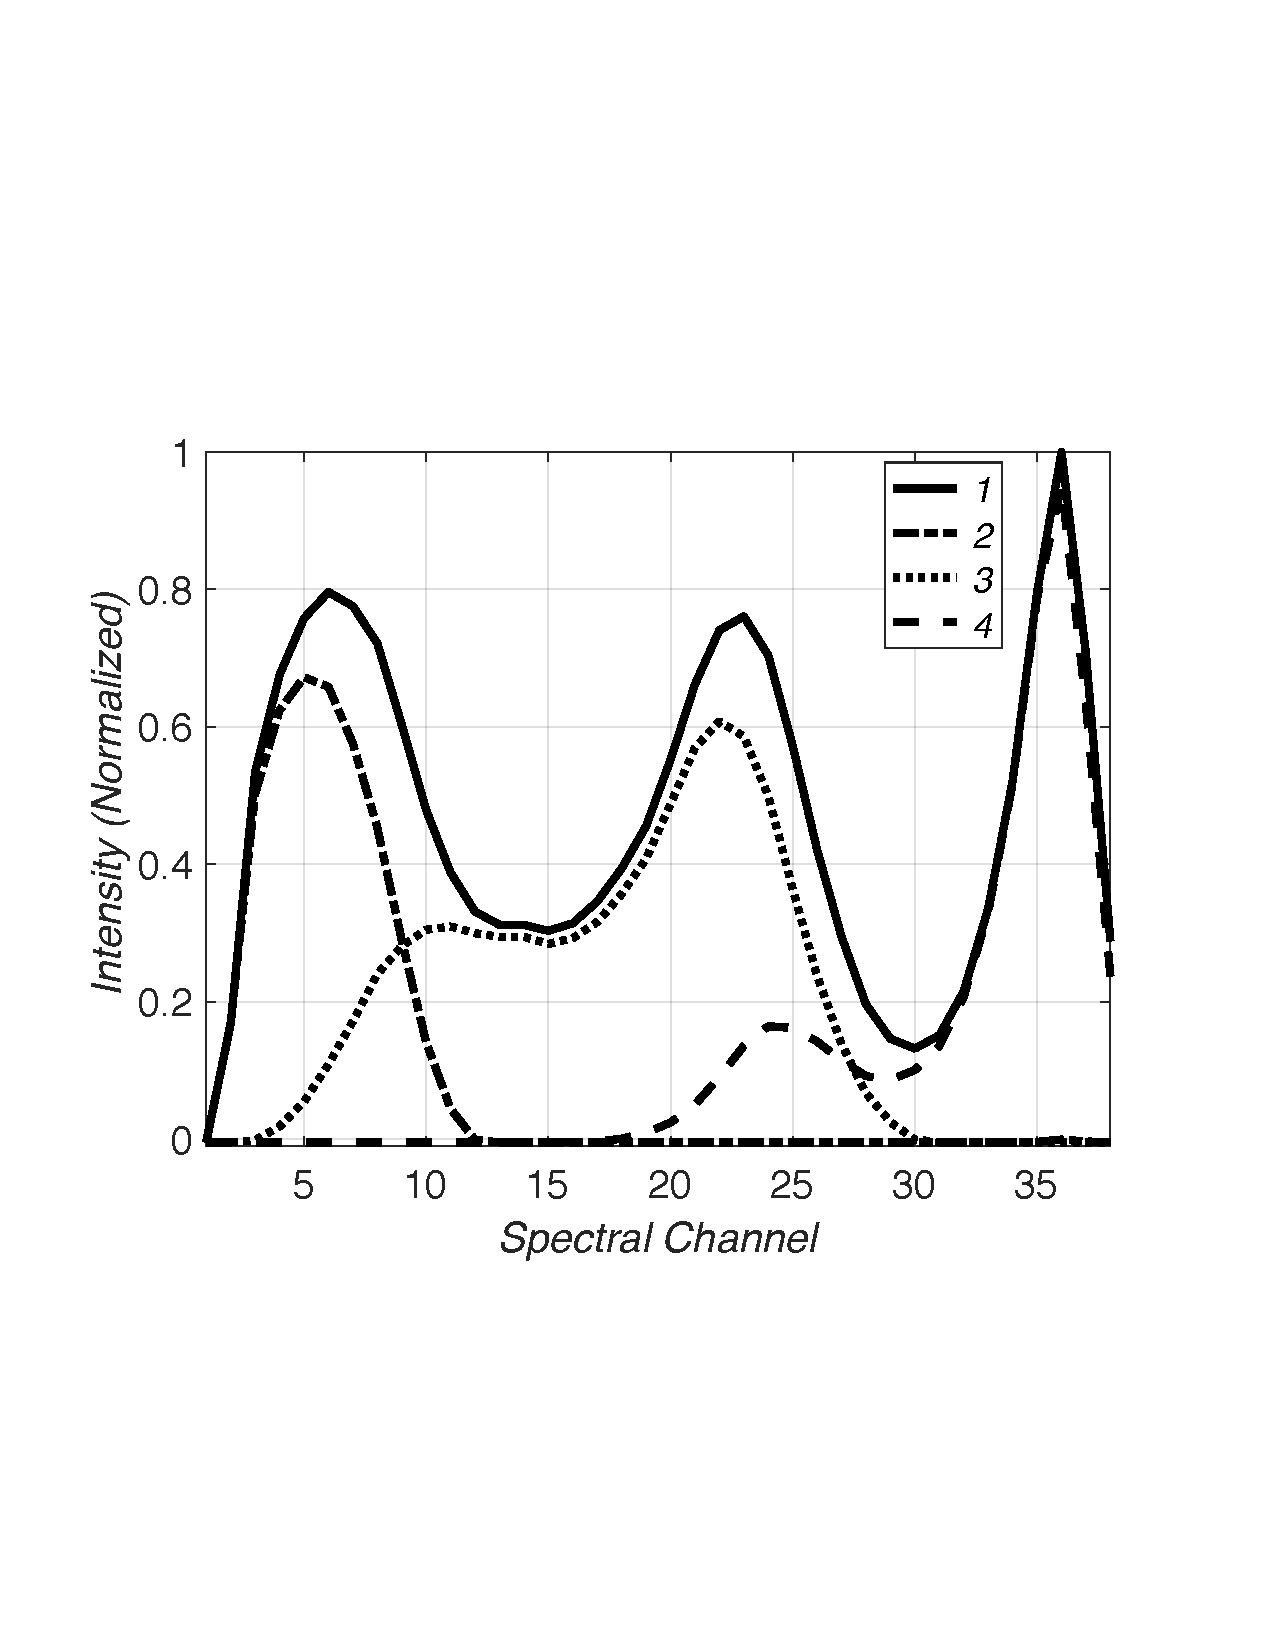
\includegraphics[scale=0.845]{afssicSpecLib}\\
	\captionof{figure}[Four class spectral library used for the AFSSI-C experiment.]{The spectral library consists of four spectral classes: the white, red, green, and blue of the LED monitor.}
	\label{fig:afssicSpecLib}
\end{figure}


% Plot of the UofA Symbol
\begin{figure}[htb]
	\centering
	
\includegraphics[scale=0.90]{afssicUofAsource}\\
	\captionof{figure}[Four class spectral source used for the \gls{afssi-c} experiment]{Four class spectral source used for the AFSSI-C experiment.}
	\label{fig:afssicUofAsource}
\end{figure}

\subsection{Hardware}

Certain considerations were made before fabrication and assembly of the experimental \gls{afssi-c} system. Here we outline some of the design decisions and consequences of those decisions.

Lenses are off-the-shelf achromatic doublets to avoid the need for custom fabrication. This also limited the degrees of freedom in the optical design, requiring the design focal lengths to match available lenses. A compact, fixed focal length, lens (Edmund Optics Stock No. 58-001, f = 12mm) is used as an objective lens, relaying the object onto an intermediate image plane. A fast entrance optic is needed to meet the layout and magnification requirements. Referring to Fig. 1, lenses 1 and 4 are 75 mm focal length achromatic doublets with a 50 mm diameter (Edmund Optics Stock No. 49-291), and lenses 2 and 3 are 150 mm focal length achromatic doublets with 25 mm diameter (Edmund Optics Stock No. 47-643). 

For a repeatable, updatable synthetic datacube source, we use an LED display (Dell P2311H LED monitor with $248  \mu m $ pixel pitch). Though this limits the spectra we are able to generate, it still allows for programmable spectra at every spatial location. The center $1080\times 1080$ pixels are used to generate the source spectral datacubes. Spectra consist of combinations of the RGB monitor colors.

The design spectral range is 425-625nm; filters were placed in the collimated space to attenuate light outside of this range. The system is designed for 38 spectral channels, resulting in roughly 5nm/spectral channel. The system magnification to the \gls{dmd}, which then dictates the lateral spread allowed per spectral channel, requires custom 0.10 lines $\mu m$ holographic blaze gratings as the dispersive elements, fabricated by Wasatch Photonics. The gratings are designed to minimize diffraction in all the orders except the first order. 

The \gls{dmd} is a Texas Instruments DLP Discovery 4100 \gls{dmd} development kit, with the DLP9500 0.95" 1080p \gls{dmd} chipset. The \gls{dmd} has $1080\times 1920$ $10.8 \mu m $ mirrors on the array, and the mirrors pivot $ 12 $ degrees on a diagonal axis. The \gls{dmd} is oriented such that the bottom of the array is parallel to the optical table, which forces the second arm of the \gls{afssi-c} to rise off the optical table at an angle of $17.5 $ degrees; this orientation was chosen so that the mirrors would be oriented as squares rather than diamonds. While the periodic structure of the \gls{dmd} can produce strong diffraction for certain types of illumination, no diffraction effects are observed in the \gls{afssi-c} as the light striking the \gls{dmd} is highly incoherent. 

An SBIG ST-10XME detector with a $2184 \times 1472$, 6.8 $ \mu m $ pitch CCD array is used as the detector array. Because of the angle of the optical axis at the detector, a goniometer was constructed using a rapid prototyping 3D printer to facilitate easy alignment of the CCD array.

Because we are interested in a quantitative system analysis, we compare measurements on the discretized detector to what was projected by our discretized source. The layout dimensions, component pixel size, and lens design were tuned to yield pixel groups---referred to here as system pixels---at each component that are an integer number of the component pixel, or in the case of the \gls{dmd}, integer number of mirrors. We therefore have the following system pixel dimensions: $16 \times 16$ pixels on the source, $8 \times 8$ \gls{dmd} mirrors, and $12 \times 12$ pixels at the detector.

Once the optical layout was finalized, the physical system was designed in SolidWorks. The lens mounts, detector mount, \gls{dmd} mount, beam dump, and locating plates were then fabricated on a Eden 350 rapid prototyping 3D printer.

Light baffling is utilized to shield the system from ambient light as well as stray light within the system. A baffling structure was designed and printed to surround the detector, with smaller baffling elements to attenuate stray light around the optical paths.


\subsection{Calibration}


As previously mentioned in~\cite{Dunlop:COSI2013}, calibration is fundamental for the functioning of a computational imaging system as the \gls{afssi-c}. Here we will elaborate on the derived challenges.

A measurement at the detector must be compared to the source to assess system performance, but the \gls{dmd} geometry creates a tilted object plane for the second arm of the \gls{afssi-c}. The \gls{dmd} plane is normal to the optical axis of the first arm, but it is at an angle (equal to twice the tilt of the mirrors on the diagonal) to the second arm. We can think of the \gls{dmd} plane as the object for the second arm of the system. This object is extended along the optical axis of the second arm, which causes keystone distortion at the detector as explained by the Scheimpflug condition \cite{ModernOpticalEngineering}. The distortion is rectified by a mapping routine which creates fiducial markers on the source. The points are registered to the corresponding image on the detector, and a lookup table can then be used to map detector pixels to the source locations.

The optical system has aberrations, and there are intensity variations across the measured ROI of the source. The system is therefore calibrated for spectral response. This is done any time physical adjustments to the system have been made. System calibration involves activating each of the available colors on the source, and then sweeping a single column of `on' system pixels (i.e., angled to send light to the detector) across the \gls{dmd}. A datacube consisting of the spectral response at each spatial location is compiled from the measurements. Knowledge of the spectral response of the system is used to accommodate aberrations and imperfect recombination of the spectral signal at the second grating.

Finally, a map of the source brightness is determined at the beginning of each experiment to account for spatial variations in the spectral throughput. This map is created by turning the entire \gls{dmd} to `on' and measuring the intensity at each spatial location from a white source. Subsequent measurements rely on this flat field measurement to accommodate for the spatially varying illumination response of the system.

\subsubsection{Spatial Calibration}

\subsubsection{Spectral Calibration}

\subsubsection{Noise Model Calibration}

\section{Experimental Results}


Figure~\ref{fig:video} presents a snapshot of a video (see \textbf{Visualization} 1) comparing system performance at different TSNR levels. As the classification difficulty increases, the system takes longer to correctly classify. However, the \gls{afssi-c} feature-design process intelligently adjusts the codes to focus attention on uncertain spatial locations

 \begin{figure}[htb]
  \centering
  % Requires \usepackage{graphicx}
  \includegraphics[scale=0.40]{video}\\
  \caption{Frame from a movie (see \textbf{Visualization} 1) showing experimental results for three different levels of TSNR, over the course of 30 measurements. The left column is a depiction of the \gls{dmd} code, center is the output from the detector, and the right is the classification decision at the current measurement.}\label{fig:video}
\end{figure}

Figure~\ref{fig:SIMmultiTSNR} shows the comparison between the \gls{afssi-c} system experiment results and the simulated values. The simulated and experimental data are the average of multiple runs, i.e., 30 simulations and 10 experiments, for each of the four TSNR values representing octaves of classification difficulty (0, -3, -6, and -9dB TSNR).
%
%Experimental data with simulation
\begin{figure}[htb]
 	\centering
  	% Requires \usepackage{graphicx}
  	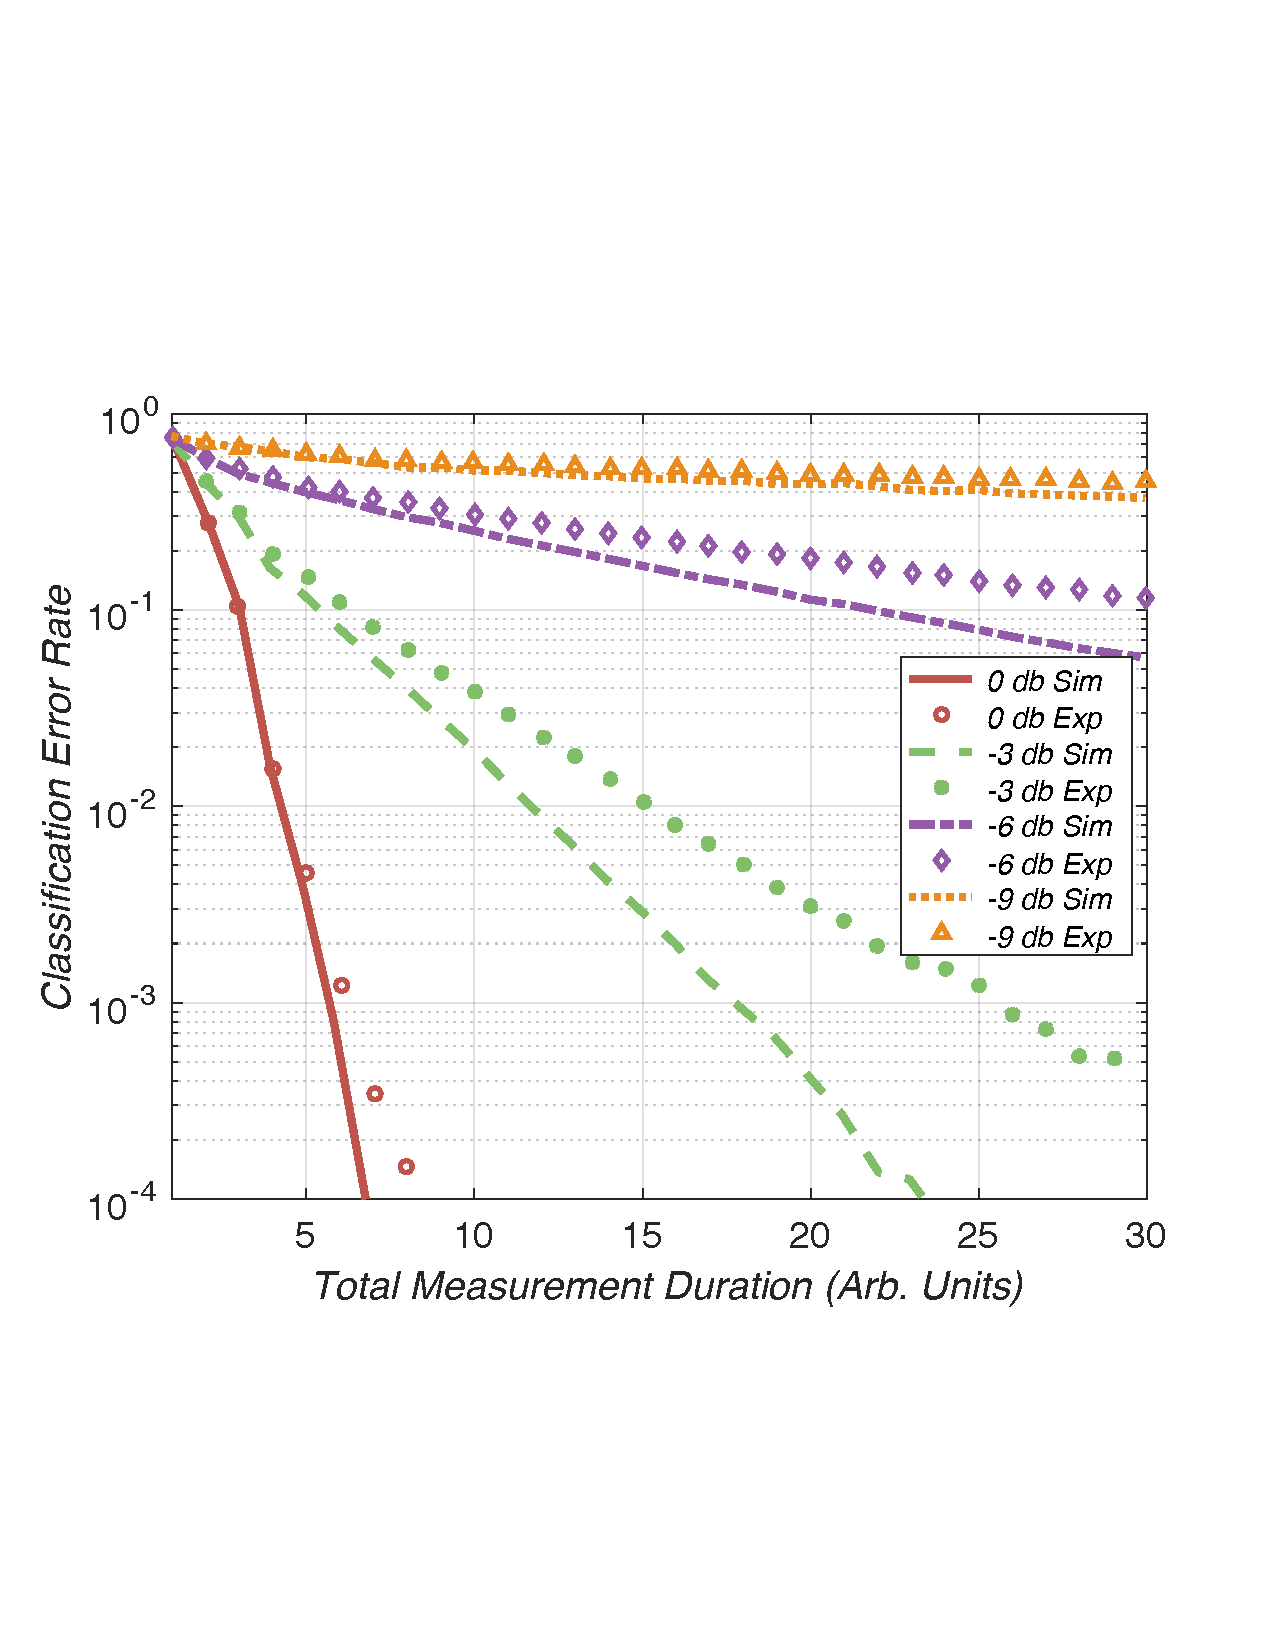
\includegraphics[scale=0.76]{afssicExpVsSim}\\
  	\caption{Comparison of the AFSSI-C experimental system results to the simulation results for multiple TSNR levels by plotting the classification error versus measurement. Shown are repeated experiments of a $64 \times 64 \times 38$ spectral datacube and a 4-class library.}\label{fig:SIMmultiTSNR}
\end{figure}
%
Figure \ref{fig:SIMmultiTSNR} shows good agreement between the  simulated and measured classification accuracy. This agreement allows us to compare the performance of the \gls{afssi-c} with traditional systems via simulation. We can then assess the gain in performance over these traditional scanning systems.

Figure~\ref{fig:SIM0TSNR} compares the \gls{afssi-c} to traditional scanning spectral imaging systems. It also compares different feature design modalities. To test feature designs, the adaptive, joint-pPCA designed features are compared to static, pseudo-random features. The traditional systems that were investigated as simulations are the pushbroom, whiskbroom, and tunable filter systems. The performance of the simulated traditional systems follows intuition---a whiskbroom system has to sweep over all 4096 spatial locations, while the pushbroom and tunable filter system only make 64 and 38 scanning steps, respectively. This explains the greater SNR and hence greater classification accuracy of the tunable filter system, with the whiskbroom system being least accurate of the three. Note that the sequential nature of the measurements in the \gls{afssi-c} limits its applicability to those scenes which are slowly varying with respect to the time needed to achieve a desired classification accuracy.

In this manuscript, we are explicitly considering the case where the spectral library is completely known---there are no \lq nuisance parameters\rq{}  such as amplitude variations of the spectra---and we are investigating the performance of the \gls{afssi-c} in this baseline scenario. However, there do exist methods for addressing nuisance parameters in Bayesian inference schemes~\cite{hernandez2014mind, hong2003classification}, which could be incorporated into the design and inference framework of the \gls{afssi-c}. Alternatively, a single uncoded measurement would capture the total signal energy at each spatial location and the library could be locally normalized to the appropriate value prior to proceeding with the algorithm described here.


%Simulation Data with Traditional Systems
\begin{figure}[htb]
  \centering
  % Requires \usepackage{graphicx}
  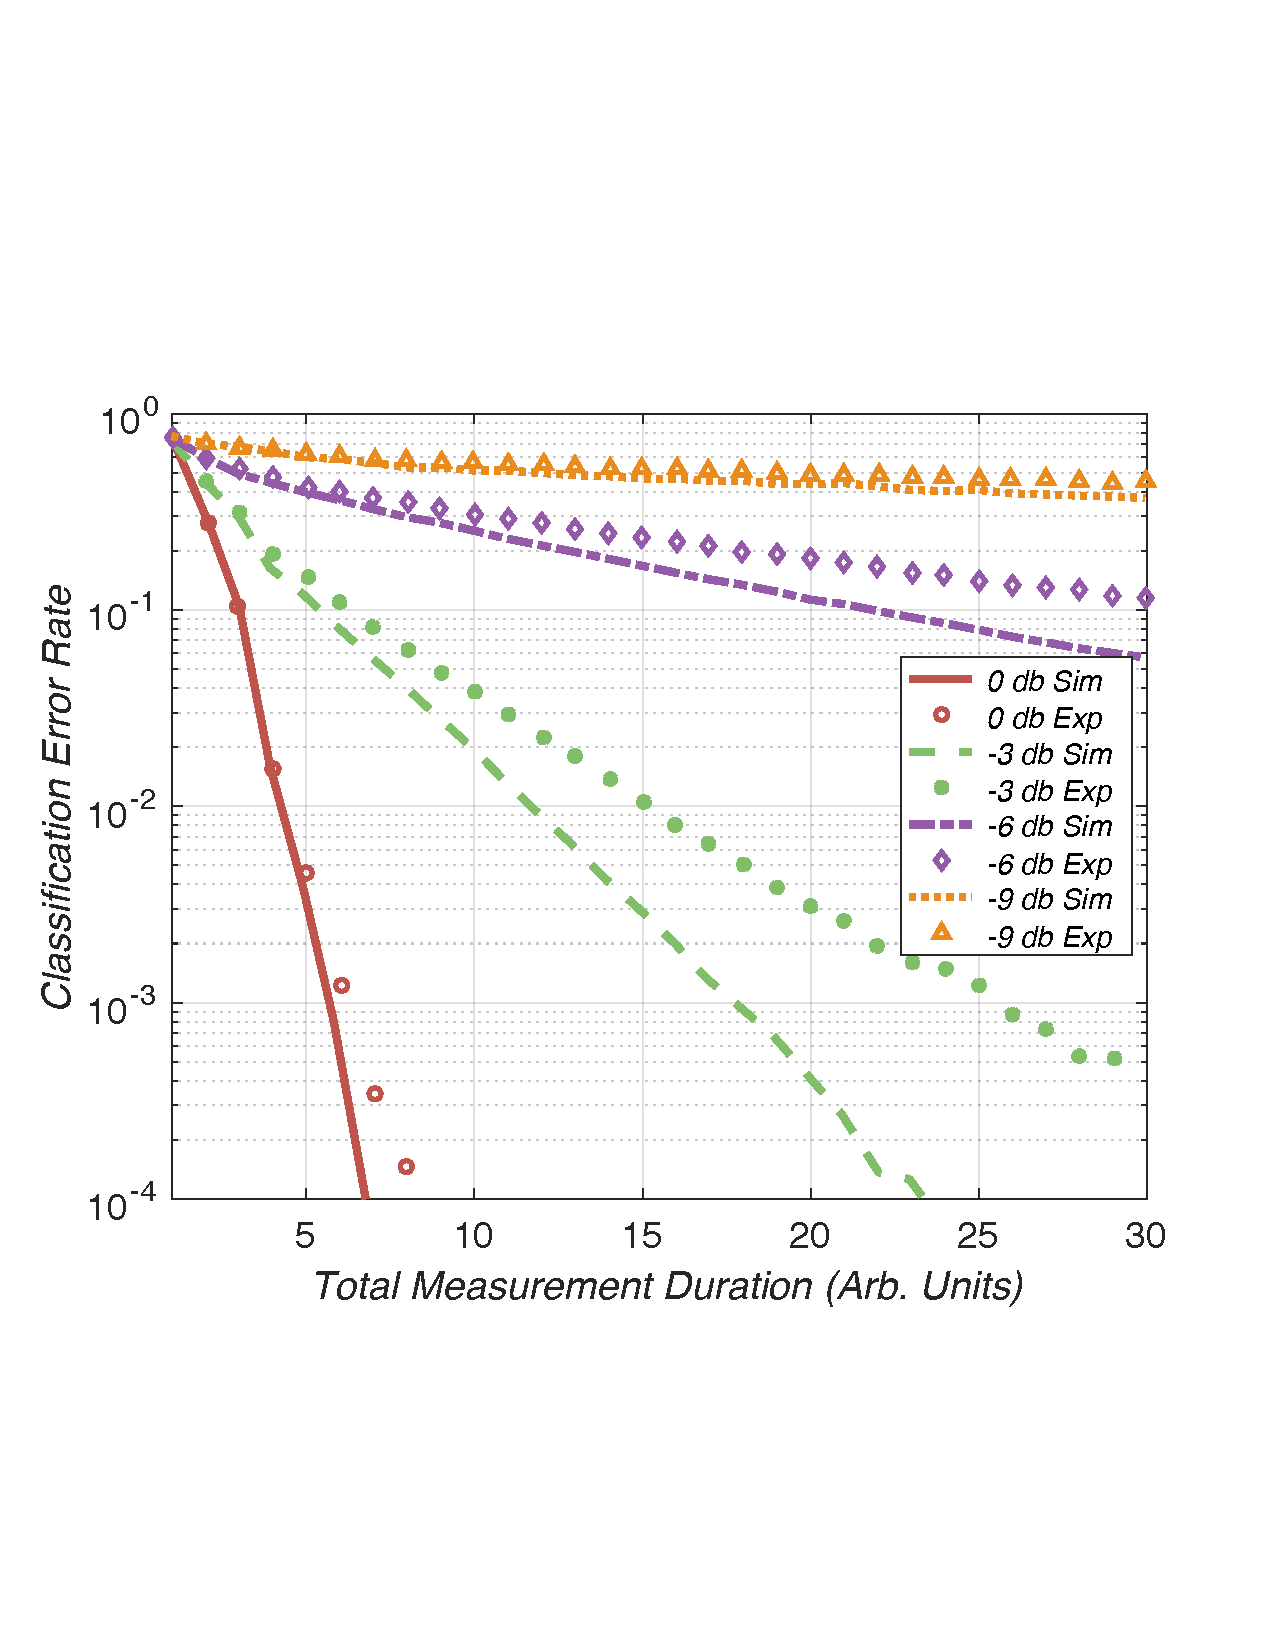
\includegraphics[scale=0.7]{afssicExpVsSim}\\%old file was NewTradCompLongRev2
  \caption{Simulation comparing the classification performance for different measurements at TSNR = 0 for different systems: the \gls{afssi-c} with designed features (joint pPCA), the \gls{afssi-c} with random features, the traditional pushbroom imager, the traditional tunable filter imager, and the traditional whiskbroom imager. The input is a $64 \times 64 \times 38$ spectral datacube with a 4-class library.} \label{fig:afssicExpVsSim}
\end{figure}


There are a number of phenomena which give the \gls{afssi-c} an advantage over traditional systems. When comparing the \gls{afssi-c} system with joint-pPCA designed features to traditional systems at the 5\textsuperscript{th} measurement in Fig. \ref{fig:afssicExpVsSim}, we see that the classification accuracy improves by 250$\,\times$. This improvement in performance is attributed to a combination of factors such as the open aperture architecture of the \gls{afssi-c} design, lack of scanning, and adaptivity. 

Figure~\ref{fig:afssicExpVsSim} also demonstrates the benefit of using joint-pPCA to design spectral features that discriminate between the possible hypothesis spectra. Looking again at the 5th measurement, we see a 100$\,\times$ performance gain relative to static, pseudorandom coding. The performance curve for the random coding case is generated by directly classifying from the acquired measurements using an identical Bayesian inference framework. The information processing inequality of information theory~\cite{cover2012elements} guarantees us that the alternative approach of classifying after datacube reconstructions can do no better than direct classification. Thus, the separation of these two curves represents the true performance improvement arising from adaptive measurement, while the separation between the static-coded curve and the traditional systems represents the performance improvement arising from the increased open aperture.  Moreover, we expect further improvement in classification accuracy for larger systems as the traditional systems become even more starved for light, having to sweep through even larger spatial arrays. In all, these simulated results indicate that there is great potential for the \gls{afssi-c} system to outperform traditional systems where classification is the desired result of the analysis.


\section{Conclusion}

In this chapter, I discussed the practical considerations of direct spectral classification using the \gls{afssi-c}, a spectral imager classifier that utilizes adaptive spectral features in a resource-lean configuration. We are able to show multiple order-of-magnitude improvement in classification accuracy compared to traditional spectral imaging systems when the noise in the system is equal to the minimum separation between the library spectra, by employing a robust system simulation corroborated with experimental results. By taking advantage of its adaptiveness, the \gls{afssi-c} performance with designed features also achieves multiple order-of-magnitude improvement over a random feature implementation. These adaptive features are designed via Bayesian inference and a novel joint-probabilistic PCA approach, which drives the measurement decision evolution to boost the discrimination ability between spectra candidates at every spatial location. 

%The system was designed with off-the-shelf lenses, though custom holographic gratings were required for the desired spectral bandwidth per channel. Design decisions led to architecture based requirements such as keystone distortion correction. Measuring system performance is possible thanks to a repeatable source spectral datacube generated using a LED monitor, and detector mapping that traces the measurements at each pixel back to the source.

Direct classification is a useful modality for many of the applications of spectral imaging. By making measurements of an encoded datacube instead of explicit measurement of every element, huge performance gains are realized. It is reasonable to imagine the \gls{afssi-c} system being of great benefit to a number of industries that rely on \textit{in situ} material classification. Further work is underway to test the system with larger spectral libraries, as well as a second generation system based on a transmissive spatial light modulator (SLM). Using a transmissive SLM will reduce keystone distortion, and simplify the optical path.
